\newpage
\subsection{Using stochastic gradient descent for regression}
In this recipe, we'll get our first taste of stochastic gradient descent. We'll use it for regression
here, but for the next recipe, we'll use it for classification.
\subsubsection{Getting ready}
Stochastic Gradient Descent (SGD) is often an unsung hero in machine learning.
Underneath many algorithms, there is SGD doing the work. It's popular due to its simplicity
and speed—these are both very good things to have when dealing with a lot of data.
The other nice thing about SGD is that while it's at the core of many ML algorithms
computationally, it does so because it easily describes the process. At the end of the day,
we apply some transformation on the data, and then we fit our data to the model with
some loss function.
\subsubsection{Implementation} % How to do it…
If SGD is good on large datasets, we should probably test it on a fairly large dataset:
>>> from sklearn import datasets
>>> X, y = datasets.make_regression(int(1e6))
# Just in case the 1e6 throws you off.
>>> print "{:,}".format(int(1e6))
1,000,000
%===========================================================================================%
%% Premodel Workflow
%% 52
It's probably worth gaining some intuition about the composition and size of the object.
Thankfully, we're dealing with NumPy arrays, so we can just access nbytes. The built-in
Python way to access the object size doesn't work for NumPy arrays. This output be system
dependent, so you may not get the same results:
>>> print "{:,}".format(X.nbytes)
800,000,000
To get some human perspective, we can convert nbytes to megabytes. There are roughly
1 million bytes in an MB:
>>> X.nbytes / 1e6
800.0
So, the number of bytes per data point is:
>>> X.nbytes / (X.shape[0]*X.shape[1])
8
Well, isn't that tidy, and fairly tangential, for what we're trying to accomplish; however,
it's worth knowing how to get the size of the objects you're dealing with.
So, now that we have the data, we can simply fit a SGDRegressor model:
>>> from sklearn import linear_model
>>> sgd = linear_model.SGDRegressor()
>>> train = np.random.choice([True, False], size=len(y), p=[.75, .25])
>>> sgd.fit(X[train], y[train])
SGDRegressor(alpha=0.0001, epsilon=0.1, eta0=0.01,
fit_intercept=True, l1_ratio=0.15,
learning_rate='invscaling', loss='squared_loss',
n_iter=5, penalty='l2', power_t=0.25, random_state=None,
shuffle=False, verbose=0, warm_start=False)

So, we have another "beefy" object. The main thing to know now is that our loss function is
squared_loss, which is the same thing that occurs during linear regression. Also worth
noting is that shuffle will generate a random shuffle of the data. This is useful if you want to
break a potentially spurious correlation. With fit_intercept, scikit-learn will automatically
include a column of ones. If you like to see more through the output of the fitting, set
verbose to 1.
%===========================================================================================%
%-- Chapter 1
%% - 53
We can then predict, as we previously have, using scikit-learn's consistent API:

\begin{figure}
\centering
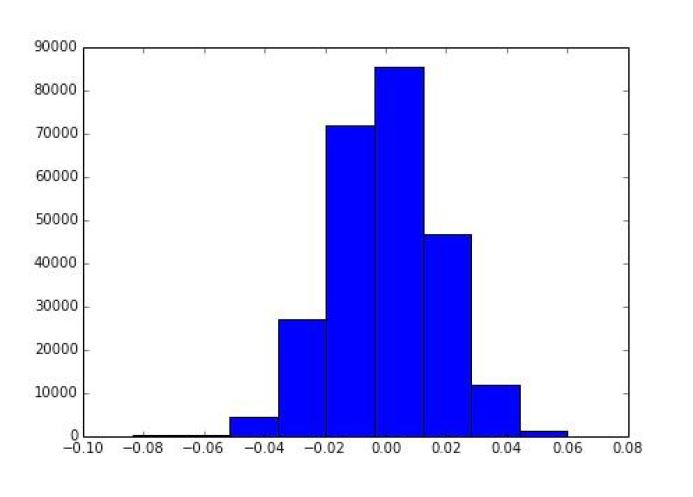
\includegraphics[width=0.7\linewidth]{SKL19-SGD-histogram}
\caption{}
\label{fig:SKL19-SGD-histogram}
\end{figure}

You can see we actually got a really good fit. There is barely any variation and the histogram
has a nice normal look.

How it works…
Clearly, the fake dataset we used wasn't too bad, but you can imagine datasets with larger
magnitudes. For example, if you worked in Wall Street on any given day, there might be two
billion transactions on any given exchange in a market. Now, imagine that you have a week's
or year's data. Running in-core algorithms does not work with huge volumes of data.
The reason this is normally difficult is that to do standard gradient descent, we're required to
calculate the gradient at every step. The gradient has the standard definition from any third
calculus course.

The gist of the algorithm is that at each step we calculate a new set of coefficients and
update this by a learning rate and the outcome of the objective function.
In pseudo code, this might look like the following:
>>> while not_converged:
w = w – learning_rate*gradient(cost(w))
%===========================================================================================%
%% Premodel Workflow
%% 54
The relevant variables are as follows:
\begin{itemize}
\item w: This is the coefficient matrix.
\item learning_rate: This shows how big a step to take at each iteration. This might
be important to tune if you aren't getting a good convergence.
\item gradient: This is the matrix of second derivatives.
\item cost: This is the squared error for regression. We'll see later that this cost function
can be adapted to work with classification tasks. This flexibility is one thing that
makes SGD so useful.
\end{itemize}
This will not be so bad, except for the fact that the gradient function is expensive. As the
vector of coefficients gets larger, calculating the gradient becomes very expensive. For each
update step, we need to calculate a new weight for every point in the data, and then update.
The stochastic gradient descent works slightly differently; instead of the previous definition
for batch gradient descent, we'll update the parameter with each new data point. This data
point is picked at random, and hence the name stochastic gradient descent.
%===========================================================================================%
